\documentclass[../../../../main.tex]{subfiles}

\begin{document}

\section*{京都大学 1984年 前期}
\begin{flushright}
120/120分
\end{flushright}
\begin{center}
\begin{tabular}{|c|l|c|c|c|}
\hline
& & 計 & 思 & 統 \\ \hline
\fbox{1} & & & & \\ \hline
\fbox{2} & 関数 & B & D & D \\ \hline
\fbox{3} & 多変数 & B & B & B \\ \hline
\fbox{4} & 多変数 $\star(1)$ & B & C & B \\ \hline
\fbox{5} & 確率 $\star$ & C & C & C \\ \hline
\fbox{6} & 関数 & A & A & A \\ \hline
\end{tabular}
\end{center}

\subsection*{第1問}
% 空白のページ

\subsection*{第2問}
[解]
(1) $f(x+2\pi) = \sin(\sin(x+2\pi)) = \sin(\sin x) = f(x)$から, $f(x)$は周期関数である. 以下, 周期が$2\pi$であることを示す.
$0 < c < 2\pi, \ f(x+c) = f(x)$をみたす$c$があるとすると
$$ \sin(x+c) = \sin x + 2n\pi, \ -\sin x + (2n+1)\pi \quad (n \in \mathbb{Z}) $$
と表せるが, $-1 \le \sin(x+c), \sin x \le 1, \ \pi \fallingdotseq 3.14$から, これらをみたす$n$は$0$のみである.
$$ \sin(x+c) = \pm \sin x $$
これを任意の$x$でみたす$c \ (0 < c < 2\pi)$は存在せず, 矛盾 \dots $\star$
よって周期は$2\pi$である. \hfill (終)

\begin{flushright}
$\left[\text{(1), (2)は} -\frac{\pi}{2} < \sin x < \frac{\pi}{2} \text{を言うと早いか (by 新)}\right]$
\end{flushright}

(2) (1)と同じく, $c = 2\pi$とすれば$f(x)$は周期関数であるから, 以下周期が$2\pi$であることを示す. $0 < c < 2\pi, \ f(x+c) = f(x)$をみたす$c$があるとすると
$$ \cos(\sin(x+c)) = \cos(\sin x) $$
$$ \cos(x+c) = \cos x + 2n\pi, \ -\cos x + 2n\pi \quad (n \in \mathbb{Z}) $$
$-1 \le \cos(x+c), \cos x \le 1$から, $n=0$で
$$ \cos(x+c) = \pm \cos x $$
これを任意の$x$でみたす$c$は存在せず, 矛盾. よって周期は$2\pi$である. \hfill (終)

(3) $f(x+c) = f(x)$をみたす$c \ (0 < c)$が存在するとする. $x=0$での成立が必要で,
$$ \sin c^3 = \sin 0 = 0 $$
$$ \therefore c^3 = n\pi \quad (n \in \mathbb{N}) $$
とおける. さらに, $0 < x < \sqrt[3]{\pi}$の時, $f(x) \neq 0$だから$c < x < c + \sqrt[3]{\pi}$でも$f(x) \neq 0$であることが必要だが, $x = \sqrt[3]{(n+1)\pi}$はこれをみたし, $f(\sqrt[3]{(n+1)\pi}) = 0$だから矛盾. よって$f(x)$は周期関数ではない. \hfill (終)

\subsection*{第3問}
[解] $P$は$\begin{pmatrix} 2 \\ 2t \end{pmatrix}, Q\begin{pmatrix} 1 \\ t \end{pmatrix}$から,
$PQ : \frac{1}{2}x - (t+1)\cdot\frac{1}{2}t - (y-t) = 0$
とおける. セイリして
$$ t^2 - xt + y = 0 \quad \cdots \text{\textcircled{1}} $$
をみたす$t \in \mathbb{R}$が存在するので, 判別式$D$として$D \ge 0$.
$$ x^2 - 4y \ge 0 $$
これを図示して, 右図斜線部.
\begin{center}
\begin{tikzpicture}
    \draw[->] (-2,0) -- (2,0) node[right] {$x$};
    \draw[->] (0,-1) -- (0,2) node[above] {$y$};
    \draw[domain=-2:2, smooth, variable=\x] plot ({\x}, {0.25*\x*\x}) node[right] {$y=\frac{1}{4}x^2$};
    \fill[pattern=north east lines] (-2,1) -- plot[domain=-2:2] (\x,{0.25*\x*\x}) -- (2,1) -- cycle;
    \node at (0.2,-0.2) {O};
\end{tikzpicture}
\end{center}

(2) \textcircled{1}から
$y = f(t) = -t^2 + xt \quad (0 \le t \le 1, \ t-1 \le x \le t+1)$
をみたす$(x,y)$をもとめる. $x=X$と固定し, 右辺$g(t)$の値域をもとめる. $(X-1 \le t \le X+1)$ 右図から
$$
\begin{cases}
g\left(\frac{X}{2}\right) \ge y \ge g(1) & (0 \le X \le 2) \\
g(0) \ge y \ge g(X+1) & (-1 \le X \le 0)
\end{cases}
$$
だから$X$をうごかして
$$
\begin{cases}
-x-1 \le y \le 0 & (-1 \le x \le 0) \\
x-1 \le y \le \frac{1}{4}x^2 & (0 \le x \le 2)
\end{cases}
$$
より, この領域は右図斜線部 (境界含む) で, もとめる面積は
\begin{align*}
S &= \frac{1}{2} \cdot 1 \cdot 1 + \int_0^2 \left(\frac{1}{4}x^2 - x + 1\right) dx \\
&= \frac{1}{2} + \frac{1}{3} \cdot \frac{1}{4} \cdot 2^3 \\
&= \frac{7}{6} \quad \text{\#}
\end{align*}

\begin{center}
\begin{tikzpicture}
    \draw[->] (-2,0) -- (3,0) node[right] {$x$};
    \draw[->] (0,-2) -- (0,2) node[above] {$y$};
    \draw[domain=0:2, smooth, variable=\x] plot ({\x}, {0.25*\x*\x}) node[right] {$y=\frac{1}{4}x^2$};
    \draw (-1,0) -- (0,-1) node[below right] {$-1$};
    \draw (0,-1) -- (2,1);
    \node at (2,1) [below right] {$y=x-1$};
    \fill[pattern=north east lines] (-1,0) -- (0,-1) -- (2,1) -- plot[domain=2:0] (\x,{0.25*\x*\x}) -- cycle;
    \node at (-1,0) [above left] {$-1$};
    \node at (2,0) [below] {$2$};
\end{tikzpicture}
\end{center}

\subsection*{第4問}
[解] (1) (与式左辺) $= u \overrightarrow{AB} + w \overrightarrow{AC} + (u-v-w) \overrightarrow{OA}$ である.
$\overrightarrow{OA}, \overrightarrow{OB}, \overrightarrow{OC}$ はどの2つも平行でないから, $u-v-w \neq 0$の時
与式左辺の表す点$O'$は$O$と異なる平面にあり不適. よって$u-v-w = 0$ だから, (1)から, 同様に
てある. このもとで, $u \overrightarrow{AB} + w \overrightarrow{AC} = 0$ となる時を考える. $\cdots \star$
$\overrightarrow{AB} = \begin{pmatrix} x_1 \\ y_1 \end{pmatrix}, \overrightarrow{AC} = \begin{pmatrix} x_2 \\ y_2 \end{pmatrix}$ とおける($\overrightarrow{AB} \not\parallel \overrightarrow{AC}$)からこの時
$$
\begin{cases}
u x_1 + w x_2 = 0 \\
u y_1 + w y_2 = 0
\end{cases}
\implies
\begin{cases}
u (x_1 y_2 - y_1 x_2) = 0 \\
w (y_1 x_2 - x_1 y_2) = 0
\end{cases}
$$
$\overrightarrow{AB} \not\parallel \overrightarrow{AC}$ から $x_1 y_2 - x_2 y_1 \neq 0$ だから $u=0, w=0$. これを$u-v-w=0$に代入して $u=0$. よって題意の時, $u=v=w=0$ である (終)
$\left[\begin{array}{l} u \overrightarrow{AB} + w \overrightarrow{AC} = (u-v-w) \overrightarrow{AO} \text{ とすれば右は自明だがそこまで} \\ \text{しなくても良い気はする} \end{array}\right]$

(2) $AP$と$BC$の交点$Q$, $BP$と$AC$の交点$R$
として点$X$に対し$\overrightarrow{AX} = \vec{x}$とおくと
$$ \vec{Q} = \frac{b}{b+c} \vec{b} + \frac{c}{b+c} \vec{c} $$
$$ \vec{R} = \frac{c}{a+c} \vec{c} $$
$P$は$AP, BC$上の点だから, $k, l \in \mathbb{R}$として
\begin{align*}
\vec{P} &= k \left( \frac{b}{b+c} \vec{b} + \frac{c}{b+c} \vec{c} \right) \\
&= (1-l) \vec{R} + l \frac{c}{a+c} \vec{c} \quad \cdots \text{\textcircled{1}}
\end{align*}
(1)と同様にして, $\vec{b} \not\parallel \vec{c}$の時, $u \vec{b} + v \vec{c} = 0 \iff u = v = 0$
だから, \textcircled{1}より
$$
\begin{cases}
1-l = k \frac{b}{b+c} \\
l \frac{c}{a+c} = k \frac{c}{b+c}
\end{cases}
\implies
\begin{cases}
k = \frac{b+c}{a+b+c} \\
l = \frac{a+c}{a+b+c}
\end{cases}
$$
\textcircled{1}に代入してからセイリして
$$ \overrightarrow{OP} = \overrightarrow{OA} + \overrightarrow{AP} = \overrightarrow{OA} + \frac{b}{a+b+c} \overrightarrow{AB} + \frac{c}{a+b+c} \overrightarrow{AC} $$
$$ = \frac{1}{a+b+c} (a \overrightarrow{OA} + b \overrightarrow{OB} + c \overrightarrow{OC}) $$
\begin{align*}
u &= \frac{a}{a+b+c} \\
v &= \frac{b}{a+b+c} \\
w &= \frac{c}{a+b+c} \quad \text{\#}
\end{align*}

\begin{center}
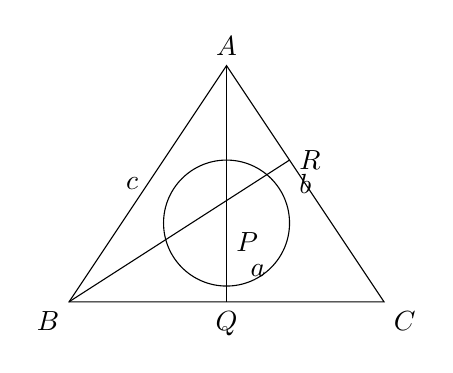
\begin{tikzpicture}
    \draw (0,0) node[below left] {$B$} -- (4,0) node[below right] {$C$} -- (2,3) node[above] {$A$} -- cycle;
    \draw (2,3) -- (2,0) node[below] {$Q$};
    \draw (0,0) -- (2.8, 1.8) node[right] {$R$};
    \node at (2,1) [below right] {$P$};
    \draw (2,1) circle (0.8);
    \node at (2.4, 0.4) {$a$};
    \node at (3, 1.5) {$b$};
    \node at (0.8, 1.5) {$c$};
\end{tikzpicture}
\end{center}

\subsection*{第5問}
[解] (1) 1回目で勝負がキマルとき. $1 \le r \le s+1$ であるから以下このもとで考える. $\cdots \text{\textcircled{1}}$
(1) 1回目に勝者が決まる確率は, $s=0$の時 $p_1 = 1$, $s \ge 1$の時, $r=1$なら $p_1 = \frac{r}{r+s}$, $r \ge 2$なら
$$ p_1 = \frac{s}{r+s} \cdot \frac{s-1}{r+s-1} \cdots \frac{s-(r-2)}{r+s-(r-2)} \cdot \frac{r}{r+s-(r-1)} $$
だから $r=1,2,3,\dots,s$の時, 一部を$A$として,
\begin{align*}
p_r - p_{r+1} &= A \cdot \frac{r}{r+s-(r-1)} - A \cdot \frac{s-(r-1)}{r+s-(r-1)} \cdot \frac{r}{r+s-r} \\
&= A r \frac{r-1}{(r+s-r)(r+s-r+1)} \ge 0 \quad \cdots *1
\end{align*}
$r=1$の時
$$ p_1 - p_2 = \frac{r}{r+s} - \frac{s}{r+s} \cdot \frac{r}{r+s-1} \ge 0 \ (\because s \ge 1) \cdots *2 $$
以上から, $p_r \ge p_{r+1}$ である. (終)

以上から $p_A \ge \frac{1}{2}$ であり, 等号が成立するのは
$1^\circ$の時の, $p_k \ge p_{k+1} \ (k=1,2 \dots 2s-1)$ とした式全てで
等号が成立する時である. この時まず$*1$での成立が必要で,
$*2$の等号が成立し, $r \ge 1, s \ge 0$から $r=1$が必要. この時 $s=1$なら坊.
$s \ge 2$の時, $*2$の等号も$r$によらず成立し, $r=1$である.
よって, もとめる条件は $r=1, s \in \text{odd}$ \hfill \#

(2) Aが勝者となるのは, $2k-1 \ (k \in \mathbb{N}, \ 1 \le 2k-1 \le s+1)$ 回目に
はじめて赤玉を引く確率で, これを$P_A$, Bが勝者となる確率を$P_B$とおくと
$1^\circ \ s=2s'-1 \ (s' \in \mathbb{N})$の時
$$
\begin{cases}
P_A = p_1 + p_3 + \dots + p_{2s'-1} \\
P_B = p_2 + p_4 + \dots + p_{2s'}
\end{cases}
$$
であり, (1)から $p_1 \ge p_2, \dots, p_{2s'-1} \ge p_{2s'}$ とした式を辺々たしあわせて
$$ P_A \ge P_B $$
これと$P_A + P_B = 1$から, $P_A \ge \frac{1}{2}$

$2^\circ \ s=2s' \ (s \in \mathbb{N}_0)$の時
$$
\begin{cases}
P_A = p_1 + p_3 + \dots + p_{2s'-1} + p_{2s'+1} \\
P_B = p_2 + p_4 + \dots + p_{2s'}
\end{cases}
$$
であり, 同様に $p_1 \ge p_2, \dots$ などとした式と $p_{2s'+1} \ge 0$から,
$$ P_A \ge P_B \quad \therefore P_A \ge \frac{1}{2} \ (\because P_A + P_B = 1) $$

$3^\circ \ s=0$の時
Aが1回目で勝利するから $P_A = 1$

\subsection*{第6問}
[解] $k \ge 0$である.
(1) $F(x) = f(x) - x$ とおくと, $F'(x) = f'(x) - 1 < 0 \ (\because (\text{ハ}))$ から, $F(x)$は
単調減少. これと $F(a) = f(a) - a \ge a - a = 0, \ F(b) = f(b) - b \le 0$
から, $F(x) = 0$をみたす$x$が $[a,b]$の中に唯1つ存在し, これが
$C_0$に他ならない. (終)

(2) 平均値の定理から $d_n \neq C_0$のとき,
$$ f(d_n) - f(C_0) = f'(p) (d_n - C_0) $$
をみたす $f'(p)$がある. (ハ)から $|f'(p)| \le k$ だから, 両辺
絶対値をとってセイリして,
$$ |d_{n+1} - C_0| \le k |d_n - C_0| \quad (\because f(d_n) = d_{n+1}, f(C_0) = C_0) $$
くり返し用いて
$$ |d_n - C_0| \le k^n |d_0 - C_0| $$
又, $d_n = C_0$の時, 明らかに成立.
以上から示された. (終)

\end{document}
